\begin{frame}
    \frametitle{Application numérique : Une alternative à l'algorithme E-M pour le mélange de gaussiennes}
    \small
    \'Echantillon $\boldsymbol{x}=\left(\boldsymbol{x}_{1}, \ldots, \boldsymbol{x}_{N}\right)$ suivant une loi 
    $f\left(\boldsymbol{x}_{i}, \theta\right)$ 
    avec des variables latentes $\boldsymbol{z}=\left(\boldsymbol{z}_{1}, \boldsymbol{z}_{2}, \dots, \boldsymbol{z}_{n}\right)$\\
    
    \begin{columns}
        \begin{column}{0.8\textwidth}
            
            \textbf{$\rightarrow$ Algorithme E-M : } Maximisation de $L(\boldsymbol{\theta} ; \mathbf{X})=p(\mathbf{x} | \boldsymbol{\theta})=\int p(\mathbf{x}, \mathbf{z} | \boldsymbol{\theta}) d \mathbf{Z}$
            $$
            L(\mathbf{x} ; \boldsymbol{\theta})=Q\left(\boldsymbol{\theta} ; \boldsymbol{\theta}^{(c)}\right)-H\left(\boldsymbol{\theta} ; \boldsymbol{\theta}^{(c)}\right)
            $$

            $$\left\{\begin{aligned}
                Q\left(\boldsymbol{\theta} ; \boldsymbol{\theta}^{(c)}\right) &=E \left[L((\mathbf{x}, \mathbf{z}) ; \boldsymbol{\theta}) | \boldsymbol{\theta}^{(c)}\right] \\
                H\left(\boldsymbol{\theta} ; \boldsymbol{\theta}^{(c)}\right) &= E\left[\sum_{i=1}^{n} \log f\left(z_{i} | \boldsymbol{x}_{i}, \boldsymbol{\theta}\right) | \boldsymbol{\theta}^{(c)}\right]
            \end{aligned}\right.$$
            $
            \boldsymbol{\theta}^{(c+1)}=\arg \max _{\boldsymbol{\theta}}\left(Q\left(\boldsymbol{\theta}, \boldsymbol{\theta}^{(c)}\right)\right)
            $ fait tendre la suite $L\left(\mathbf{x} ; \boldsymbol{\theta}^{(c+1)}\right)$ vers un max local  
            
    \end{column}

\begin{column}{0.2\textwidth}  %%<--- here
    \vspace{-0.5cm}
    \begin{figure}
        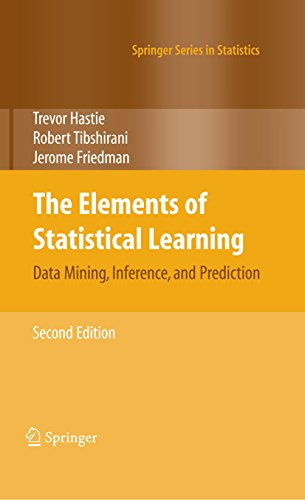
\includegraphics[width=\textwidth]{Figures/the_element.jpg}
    \end{figure}
\end{column}
\end{columns}



\end{frame}

\begin{frame}

\frametitle{Application : mélange de gaussiennes}

\vspace{-0.5cm}
\begin{columns}
    \begin{column}{0.7\textwidth}
        
        \begin{itemize}
            \item Les données $\mathbf{x}$ viennent de gaussiennes $\{ C_1,\ldots, C_M \}$ 
            %\vspace{0.5cm}
            \item $\boldsymbol{z}_{i} \in \{1,\ldots, m \}$ si un individu $i$ vient de $C_1, \ldots, C_M$
            $$ 
                \boldsymbol{x}_i |\left(\boldsymbol{z}_{i}=j\right) \sim \mathcal{N}\left(\mu_{j}, \sigma_{j}^{2}\right) \quad \mathbb{P}\left(\boldsymbol{z}_{i}=j\right)=\pi_{j} 
            $$
            $\theta=\left(\pi, \mu, \sigma^{2}\right)$ 
            \item \textbf{E-M} : maximisation de $\hat{\theta}_{\mathrm{MLE}}(x)=\underset{\theta}{\arg \max } f(x | \theta)$\\
            
            $$\ell_{\theta}(x)=\sum_{n=1}^{N} \log \left(\sum_{j=1}^{M} \pi_{j}\ \mathcal{N}_{\mu_{j}, \sigma_{j}^2}\left(x_{n}\right)\right)$$

            \item \textbf{Bayesien} estimateur $\hat{\theta}_{MMSE}(x)=E[\theta | x]$
        \end{itemize}
    \end{column}
    \begin{column}{0.3\textwidth}  %%<--- here
        \vspace{-0.5cm}
        \begin{figure}
            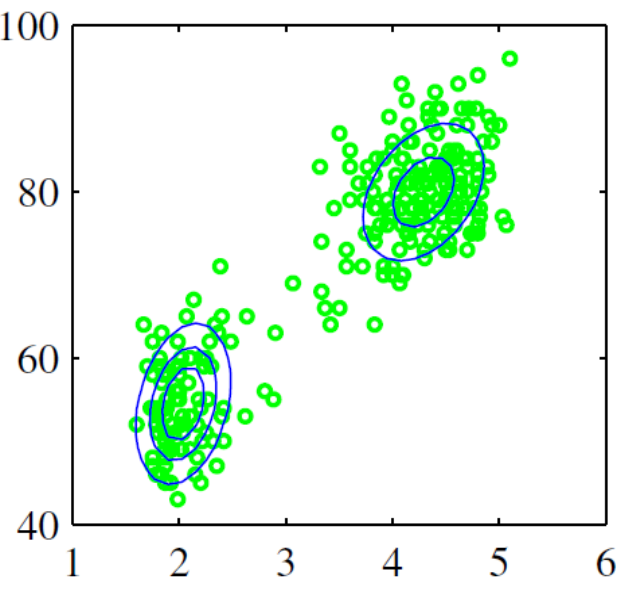
\includegraphics[width=\textwidth]{Figures/mix_gaussienne.png}
            \caption{\tiny Mélange de deux gausiennes [F. Sur, Introduction à l'apprentissage automatique]}
        \end{figure}
    \end{column}
\end{columns}

\end{frame}

\begin{frame}
    \frametitle{Application : \'Echantillonneur de Gibbs pour le mélange de 2 gaussiennes}
    Pour 2 gaussiennes:
    $\left\{\begin{aligned}
        &\boldsymbol{x}_i |\left(\boldsymbol{z}_{i}=1\right) \sim \mathcal{N}\left(\mu_{1}, \sigma_{1}^{2}\right) \quad \mathbb{P}\left(\boldsymbol{z}_{i}=1\right)=\pi_{1}\\
        &\boldsymbol{x}_i |\left(\boldsymbol{z}_{i}=2\right) \sim \mathcal{N}\left(\mu_{2}, \sigma_{2}^{2}\right) \quad \mathbb{P}\left(\boldsymbol{z}_{i}=2\right)=\pi_{2} = 1- \pi_{1}
    \end{aligned}\right.$
        \vspace{0.4cm}
        
        $\rightarrow$ On veut obtenir $\Theta = (\boldsymbol{z}, \mu) = (\boldsymbol{z_1}, \ldots,\boldsymbol{z_1},  \mu)$ \hfill($\pi, \sigma$ fixés à $\hat{\pi}, \hat{\sigma}$)
    \end{frame}

    \begin{frame}
        \frametitle{\small Application : \'Echantillonneur de Gibbs pour le mélange de 2 gaussiennes}
        \vspace{-0.5cm}
    \begin{itemize}
        \item $\Theta = (\boldsymbol{z}, \mu) = (\boldsymbol{z_1}, \ldots,\boldsymbol{z_1},  \mu)$
        \item \textcolor{beamerfooter3}{\Large $\boldsymbol{z} | \mu$} :  
        On a $p\left(\mathcal{C}_{1} | x\right)=\frac{p\left(\mathcal{C}_{1}\right) p\left(x | \mathcal{C}_{1}\right)}
        {p\left(\mathcal{C}_{1}\right) p\left(x | \mathcal{C}_{1}\right)+p\left(\mathcal{C}_{2}\right) p\left(x | \mathcal{C}_{2}\right)}$ 
        \\\vspace{0.2cm}
        Utiliser
        $\mathbb{P}\left(\boldsymbol{z}_{i}=j | \mu, \boldsymbol{x} \right)=
        { \displaystyle \frac{
            \hat{\pi}_{j}  p_{\mathcal{N}}(\boldsymbol{x}_i,\mu_{j}, \hat{\sigma}_{j})
            }{
                \hat{\pi}_{1}  p_{\mathcal{N}}(\boldsymbol{x}_i,\mu_{1}, \hat{\sigma}_{1})  +  
                \hat{\pi}_{2}  p_{\mathcal{N}}(\boldsymbol{x}_i,\mu_{2}, \hat{\sigma}_{2})
            }} \quad j \in \{ 1,2\}
            $             
        \item \textcolor{beamerfooter3}{\Large $\mu | \boldsymbol{z}$} :
        
        \begin{columns}[T]
            
            \begin{column}{0.3\textwidth}  %%<--- here
                \centering
                {\small (à priori)} \\
                \vspace{0.1cm}
                $\begin{aligned}
                    \boldsymbol{x_i} | \mu,\boldsymbol{z_i} = j & \sim \mathcal{N}\left(\mu_{j}, 1 / \hat{\tau}_j \right) \\
                    \mu_j & \sim {\mathcal{N}}\left(\mu_{0}, 1 / \tau_{0}\right) \\
                \end{aligned}$ \\
                \vspace{0.2cm}
                {\tiny $\left(\tau_j = 1 / \sigma_j^2, \ \bar{x}=\frac{1}{N} \sum_{i=0}^{N}{x_i}\right)$}
            \end{column}
            \begin{column}{0.3\textwidth}
                \centering
                {\small (à postériori)} \\
                \vspace{0.2cm}
                $\begin{aligned}
                    p(\mu_j | \boldsymbol{z}_i, \mathbf{x}) & \propto p(\boldsymbol{x} | \mu,\boldsymbol{z_i} = j) p(\mu_j)  \\
                    & \sim {\mathcal{N}}( \mu_{j_0}^{\prime}, 1 / \tau^{\prime}_{j_0}) 
                \end{aligned}$
            \end{column}
            \begin{column}{0.4\textwidth}  %%<--- here
                \centering
                {\small (= maj des coefs)} \\
                \vspace{0.1cm}
                $\begin{aligned}
                    \tau^{\prime}_{j_0} &= \tau_0 + N \hat{\tau}_j \\
                    \mu_{j_0}^{\prime} &= \frac{N\ \hat{\tau}_j\ \bar{x}+\tau_{0} \mu_{0}}{N \hat{\tau}_j+\tau_{0}} 
                \end{aligned}$
            \end{column}     
            % \begin{column}{0.14\textwidth}  %%<--- here
            %     \begin{flushleft}
                    
            %     {\tiny }
            %     \end{flushleft}
            % \end{column}     
        \end{columns}
\end{itemize}
    
\end{frame}

\begin{frame}
    \small
    \begin{exampleblock}{\'Echantilloneur de Gibbs pour une mixture gaussienne}
    \begin{enumerate}
        \item Prendre les valeurs initiales $\Theta_0 = (\boldsymbol{z}^{(0)}, \mu_{1}^{(0)}, \mu_{2}^{(0)})$, $\mu_0, \tau_0$
        \item Pour t de  à ...
            \begin{itemize}
                \item Pour $i$ de 1 à $N$ tirer \\
                {\addtolength{\leftskip}{2cm} 
                    $\boldsymbol{z}_i^{(t+1)} \in \{1, 2 \}$ avec $\mathbb{P}(\boldsymbol{z}_i^{(t+1)}=1 | \mu^{(t)}) = 
                    { \displaystyle \frac{
                    \hat{\pi}_{1}  p_{\mathcal{N}}(\boldsymbol{x}_i,\mu_{1}^{(t)}, \hat{\sigma}_{1})
                    }{
                        \hat{\pi}_{1}  p_{\mathcal{N}}(\boldsymbol{x}_i,\mu_{1}^{(t)}, \hat{\sigma}_{1})  +  
                        \hat{\pi}_{2}  p_{\mathcal{N}}(\boldsymbol{x}_i,\mu_{2}^{(t)}, \hat{\sigma}_{2})
                    }}$
                }
                \item Pour $j \in \{ 1,2\} $ \\
                Avec 
                $\tau^{\prime}_{j_0} = \tau_0 + N \hat{\tau_j} \quad \displaystyle
                \mu_{j_0}^{\prime} = \frac{N\ \hat{\tau_j}\ \bar{x}+\tau_{0} \mu_{0}}{N \hat{\tau_j}+\tau_{0}} 
                $ \\
                Tirer $\mu_{j}^{(t+1)}\ \boldsymbol{z} \sim \mathcal{N}\left(\mu_{j_0}^{\prime}, 1 / \tau^{\prime}_{j_0}\right)$
            \end{itemize}
    \end{enumerate}
   
\end{exampleblock}
\end{frame}

\begin{frame}[fragile]
    %\frametitle{\tiny Implémentation sous R}
    \vspace{-0.2cm}
    \begin{columns}
        \begin{column}{0.5\textwidth}
            
            \begin{lstlisting}[
                basicstyle=\fontsize{5}{5}\selectfont\ttfamily, %or \small or \footnotesize etc.
                captionpos=b,
                numbers = none
            ]
Z_given_mu <- function(X,Z,mu,pi_1){
    # Z variables latentes
    
    remove_i <- (c(1:length(X)) !=i) # enleve variable i
    estimate_sigma_1 <- sd(X[(remove_i & Z == 1)]) # classe 1
    estimate_sigma_2 <- sd(X[(remove_i & Z == 2)]) # classe 2 
                    
    for (i in 1:length(Z)){
                    
        proba1 <- pi_1 * dnorm(X[i],mu[1],estimate_sigma_1) / 
            (pi_1 * dnorm(X[i],mu[1],estimate_sigma_1) + 
            (1-pi_1) * dnorm(X[i],mu[2],estimate_sigma_2))

        Z[i] = sample(1:2, size=1,prob=c(proba1, 1-proba1),
            replace=TRUE)
    }
    return(Z)
}
        \end{lstlisting}
            
        \end{column}
        \begin{column}{0.5\textwidth}  %%<--- here
            
            \begin{lstlisting}[
                basicstyle=\fontsize{5}{5}\selectfont\ttfamily, %or \small or \footnotesize etc.
                captionpos=b,
                numbers = none
            ]
mu_given_Z = function(X, Z, mu_prior){
    # Z variables latentes  
    # mu_prior contient parametres loi a priori de mu

    mu = rep(0,2) ; sigma = rep(0,2)
        
    for(j in 1:2){
        
        sample_j_size = sum(Z==j) 
        sample_j_mean = mean(X[Z==j])
        sigma[j] = sd(X[Z==j]) ; precision_j = 1 / sigma[j]^2
        
        precision_post = sample_j_size * precision_j + 
            mu_prior$precision
        
            mean_post = (sample_j_mean * sample_j_size * 
            precision_j + mu_prior$mean * 
            mu_prior$precision ) / precision_post
        
        mu[j] = rnorm(1,mean_post,sqrt(1/precision_post)) # on tire mu selon la loi normale a posteriori
    }
    return(list(mu = mu, sigma = sigma))
    }
        \end{lstlisting}
    \end{column}
\end{columns}
\vspace{-0.3cm}
\begin{lstlisting}[
    basicstyle=\fontsize{5}{5}\selectfont\ttfamily, %or \small or \footnotesize etc.
    captionpos=b,
    caption={\tiny Implémentation en R},
    numbers = none
]
echantillonneur_gibbs <- function(X,N_simu){
    # X sont les donnees
    # initalisation
    .
    .
    
    for (k in 1:N_simu){ 
        
        Z <- Z_given_mu(X,Z,mu,pi_1) ; param_post <- mu_given_Z(X, Z, mu_prior)
        mu = param_post$mu
    .
    .
    .
    }
    return(list(Z, mu_1, mu_2))
}     
\end{lstlisting}
\end{frame}

\begin{frame}
    \frametitle{Simulations} \hfill \small Données : on gènere équiprobablement 1000 points à partir de 2 gaussiennes $\mathcal{N}\left(-2, 1\right), \mathcal{N}\left(-3, 0.5\right)$
    
    \centering
   
            
            \begin{figure}
                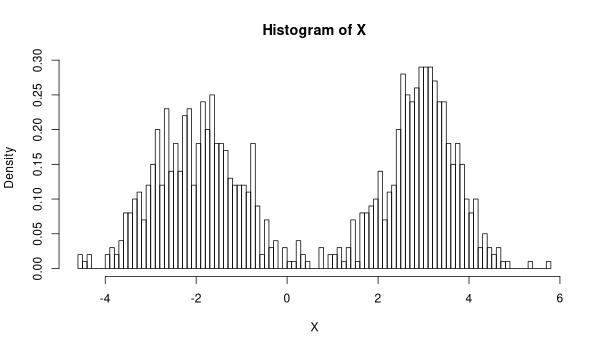
\includegraphics[width=0.55\textwidth]{../MCMC_numeric/simu_gaussian/data.png} 
            \end{figure}
   
    \vspace{-0.2cm}
    
    On prend à priori $\mu \sim \mathcal{N}\left(0, 4\right)$
\end{frame}

\begin{frame}
    \frametitle{Simulations} 
    \centering
    \small Pour 1000 itérations
    \vspace{0cm}
    \begin{columns}
        \begin{column}{0.8\textwidth}
            \begin{figure}
                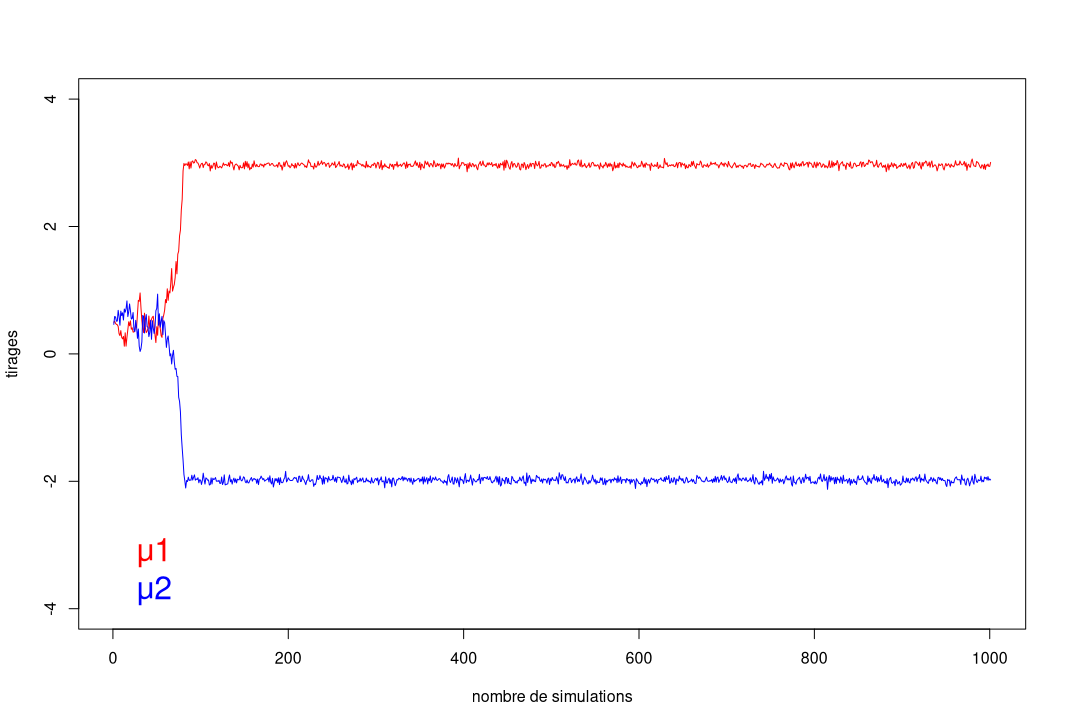
\includegraphics[width=0.8\textwidth]{../MCMC_numeric/simu_gaussian/mu.png} 
            \end{figure}
            
        \end{column}
        \begin{column}{0.2\textwidth}
            \centering
            $\rightarrow$ \textit{burn-in} de 100
        \end{column}
    \end{columns}
    \end{frame}


\begin{frame}
    \frametitle{Simulations : diagnostic de $\mu$ avec le package coda}
    \centering
    \vspace{-0.2cm}
    \begin{columns}
        \begin{column}{0.5\textwidth}
            
            \begin{figure}
                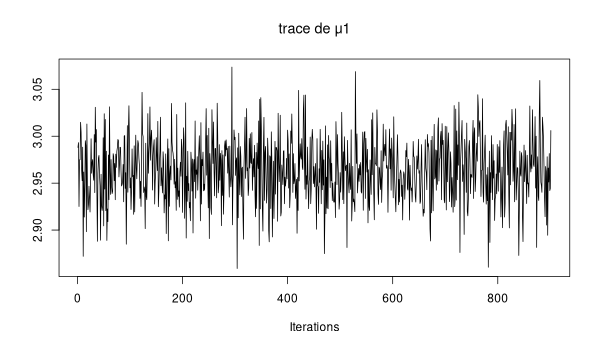
\includegraphics[width=\textwidth]{../MCMC_numeric/simu_gaussian/mu_plot_trac.png} 
            \end{figure}
        \end{column}
        \begin{column}{0.5\textwidth}

            \begin{figure}
                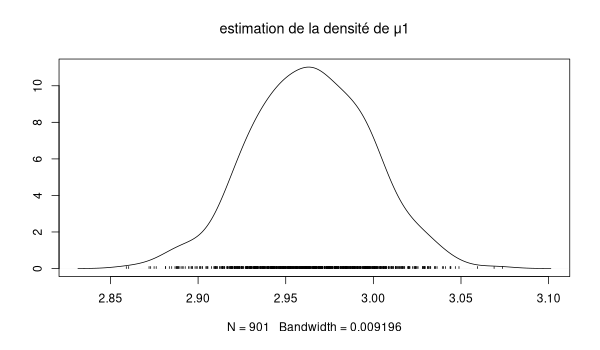
\includegraphics[width=\textwidth]{../MCMC_numeric/simu_gaussian/mu_plot_dens.png} 
            \end{figure}
        \end{column}
    \end{columns}
    (sans le \textit{burn-in})
\end{frame}
\begin{frame}
    \frametitle{Simulations : diagnostic de $\mu$ avec le package coda}

    \begin{table}[]
        \begin{tabular}{ccccc}
        \hline
        \multicolumn{1}{|l|}{variable} & \multicolumn{1}{l|}{moyenne} & \multicolumn{1}{l|}{95\% CI lower} & \multicolumn{1}{l|}{95\% CI upper} & \multicolumn{1}{l|}{vraie valeur} \\ \hline
        $\mu_1$                        & 2.963882                     & 2.899498                           & 3.032716                           & 3                                 \\ \hline
        $\mu_2$                        & -1.981757                    & -2.061083                          & -1.902244                          & -2                                \\ \hline
        \end{tabular}
        \end{table}
\end{frame}





